\documentclass{beamer}

\usepackage{helvet}
\renewcommand{\rmdefault}{\sfdefault}

\usepackage{amsmath, amsfonts, epsfig, xspace}
\usepackage{algorithm,algorithmic}
\usepackage{pstricks,pst-node}
\usepackage{multimedia}
\usepackage[normal,tight,center]{subfigure}
\setlength{\subfigcapskip}{-.5em}

\usepackage{beamerthemesplit}
\usetheme{AnnArbor}
\usecolortheme{orchid}
\usefonttheme{structurebold}

\usepackage{tikz}

% TITLE

\author[Peter J. Braam]{Peter J. Braam}

\title[Global Parallel Computing \hspace{2em}\insertframenumber/\inserttotalframenumber]
{Global Parallel Computing and Networks}

\date{Feb, 2016} %leave out for today's date to be insterted

\institute{Parallel Scientific, LLC}

\makeatletter
\newcommand\listofframes{\@starttoc{lbf}}
\makeatother

\addtobeamertemplate{frametitle}{}{%
  \addcontentsline{lbf}{section}{\protect\makebox[2em][l]{%
    \protect\usebeamercolor[fg]{structure}\insertframenumber\hfill}%
  \insertframetitle\par}%
}

\begin{document}

\begin{frame}
\frametitle{List of Frames}
\listofframes
\end{frame}


% INTERMEDIATE CONTENTS - blanked out
%\AtBeginSection[]
%{
%\begin{frame}{Contents}
%\tableofcontents[currentsection]
%\end{frame}
%}


% TITLE SLIDE
\maketitle

% CONTENT SLIDE
\tableofcontents 

% MOTIVATION & CONTENTS

\section{Introduction}

\begin{frame}{Intro}

\begin{itemize}
    \item A broad set of algorithms can be parallelized using ideas of finite geometry.  This appears to generalize important known cases.
    \item This finite geometry describes a computer network. Recent development in silicon photonics networking may make this a viable architecture.
    \item This subject matter has a very short but rather turbulent and unsuccessful commercial history. 
\end{itemize}  
\end{frame}


\section{Parallel Programming}

%SLIDE 1: Parallel Programming
\begin{frame}{Parallel Programming}
Parallel programs do one or more of the following:

\begin{itemize}
\item Execute instructions of algorithms concurrently. 
\item Use partitioned resources such as memory
\item Move data simultaneously along different links
\item Access a resource concurrently from multiple threads 
\end{itemize}

Parallelism can be a static element of the software and can be adapted dynamically.

\begin{alertblock}{Parallelism vs. Concurrency}
{\bf Parallelism:} simultaneous operations.

{\bf Concurrency:} simultaneous access to shared data.
\end{alertblock}

\end{frame}




% BLOCK HOW to make Parallel Programs?
\begin{frame}{Creating and Optimizing Parallelism}
\begin{columns}[t]
\column{0.45\textwidth}
\begin{block}{Creation}
\begin{itemize}
\item re-use data in different threads
\item partition \& use threads per partition, e.g.
\begin{itemize}
    \item vectorization
    \item tiling data
    \item nested parallelism
\end{itemize}   
\item parallelize data movement, e.g. loop unrolling
\end{itemize}
\end{block}

\column{0.45 \textwidth}
\begin{block}{Optimizing}
\begin{itemize}
    \item Decompose and create even compute load
    \item Position data to equalize and minimize data movement
    \item Decompose finely enough to keep everything busy
    \item Unroll to keep pipelines full
\end{itemize}
\end{block}
\end{columns}
\end{frame}

\begin{frame}{Parallelization tools}
\begin{itemize}
    \item Quite few tools exist handling simple cases
        \begin{itemize}
            \item macros as in OPENMP
            \item languages that compile to parallel code
            \item work load adjusters
        \end{itemize}
    \item There is a set of parallel algorithms
\end{itemize}

\begin{alertblock}{Theory is Limited}
Even for basic linear algorithms optima are not always known
\end{alertblock}
\end{frame}

\begin{frame}{Matrix Vector Multiplication: row-wise vs. Cannon}


\begin{figure}
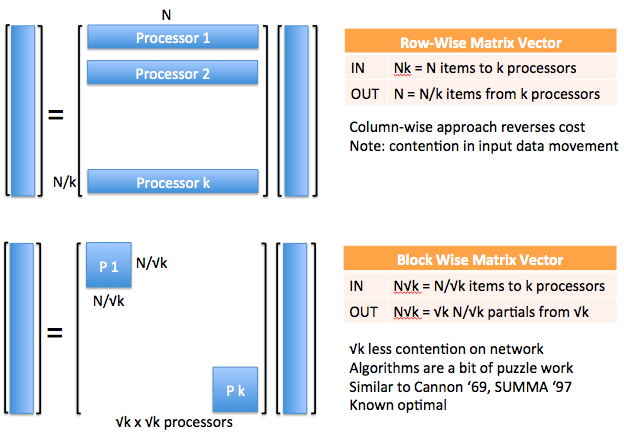
\includegraphics[scale=0.45]{row-wise-vs-cannon.png}
%\caption{Row Wise vs. Cannon Algorithm}
\end{figure}

\end{frame}

% SECTION 
\section{Finite Geometries and Parallel Algorithms}  % add these to see outline in slides


\begin{frame}{Planar Geometry and architecture}

\begin{block}{Architecture: Memory, Processor, Interconnect}
  \begin{itemize}
  \item Each {\bf point} represents a {\bf memory module} $M$
  \item Each {\bf line} represents a {\bf processor} $P$
  \item $M \in P$ {\bf iff}  $P$ is {\bf connected} to $M$
  \end{itemize}
\end{block}

\begin{block}{Geometry and Realizing Computations}
\begin{itemize}
  \item any two lines $P_1, P_2$ intersect in a point
  \item Any two points determine a line
\end{itemize}
Hence:
\begin{itemize}
    \item Any binary operation is possible two moves for input
    \item Any communication is possible, using at most one hop
\end{itemize}
{\bf Note:} We have not achieved good parallelism yet.
\end{block}
\end{frame}


\begin{frame}{Geometries of other dimensions}
\begin{block}{4D geometries - join of database tables}
\begin{itemize}
\item $(\alpha, \beta) and (\gamma, \delta)$ are an element of the join if $\beta = \gamma$.
\item Using a 4-dimensional geometry where {\bf lines represent memory modules and planes processors}.
\item The pairs determine a line 
\item Evaluate $\beta == \gamma$ on processors (planes) spanned by $\langle \alpha, \beta, \gamma \rangle$
\end{itemize}
Accumulations of ternary operations work similarly.  E.g. Gauss Elimination: $A_{ij} \leftarrow A_{ij} - \frac{A_{ik}A_{kj}}{A_{kk}}$.
\end{block}

\begin{alertblock}{Data placement vs Movement}
By placing data according to this scheme in the first place, we don't even have to move it. Here however we are more flexible on the computations we can do.
\end{alertblock}
\end{frame}

\begin{frame}{2D Parallelization}
\begin{block}{Perfect Access Patterns}
Denote the memories locations by $M$, processors by $P$. \\
A set $AP \subset M \times M \times P$ is a  {\bf perfect access pattern} if:
  \begin{itemize}
  \item If $(M_\mu, N_\nu, P_\pi) \in AP$ then $P_\pi = <M_\mu, N_\nu>$ 
  \item The two projections: $AP \rightarrow M$ are bijective (i.e. every input and ouput memory element is in a unique triple)
  \item The projection $AP \rightarrow P$ is bijective (i.e. every processor is in a unique triple)
  \end{itemize}
\end{block}
  
\begin{block}{The perfect access pattern is a {\bf global parallel instruction}}
  \begin{itemize} 
  \item There are no conflicting memory accesses
  \item All processors are used equally
  \item All network connections are used evenly
  \item The concept generalizes to other dimensions
  \end{itemize}
\end{block}
\end{frame}

\begin{frame}{Perfect and Complete Sets of Access Patterns}
\begin{block}{A set $\{ AP_i\}$ of perfect access patterns}
\begin{itemize}
\item Is {\bf complete} if it contains every pair $M_\mu, N_\nu$
\item Is {\bf perfect} if it uses all network connections evenly
\end{itemize}
\end{block}

\begin{block}{Parallel Programs}
\begin{itemize}
\item A parallel program iterates over complete sets
\item Each step in the iteration uses a perfect access pattern.
\item Perfect access patterns and perfect sequences in 2D exist
\item In 4D generally only complete sets have been found
\item The diagonal entries need special care
\end{itemize}
\end{block}
\end{frame}

\begin{frame}{Perfect Sets and Finite Projective Geometries}
\begin{block}{Finite projective spaces of dimension $d$ over a finite field $\mathbb{F}$}
  \begin{itemize}
  \item Are the set of $d+1$ dimensional subspaces of $\mathbb{F}^{d+1}$
  \item $\mathbb{F}$ is a Galois field and must have $s = p^q$ elements for a prime $p$
  \item $\mathbb{P}^2(s)$ has $N=s^2+s+1$ points and as many lines
  \item Each line contains $s+1$ points
  \item There are $s(s+1)$ ordered pairs of points on a line
  \end{itemize}
  \end{block}

\begin{block}{Creating Perfect Sequences}
\begin{itemize}
\item Perfect access patterns can be created as {\bf an} orbit of a pair $(m,n,\langle m,n \rangle) \in M \times M \times P$ under the automorphism group of $\mathbb{P}_2(s)$
\item Perfect sequences are the orbits indexed by all pairs in a line.
\item {\bf Note:} In higher dimensions perhaps only complete sequences can be found
\end{itemize}
\end{block}
\end{frame}



\begin{frame}{Finite Fields, other dimensions}

\begin{itemize}
\item There is a $d$-dimensional finite projective space for every finite field.
\item The only finite fields are the Galois fields $GF(p^q)$ where $p$ is prime and $q>0$ an integer
\item A parallel architecture can be build with memory units being the elements of $\Omega_m$ and processors elements of $\Omega_p$ if $m<p$. These would allow for parallel operations on $m+1$ arguments.
\item If $m+p = d-1$ the number of processors equals the number of memories.  Patterns appear to match d-ary operations.  
\item Architectures with more memories than processors obtain more memory bandwidth but are unconventional.  Patterns might efficiently compute encoding.
\end{itemize}
\end{frame}

\section{Architectures}

\begin{frame}{Sample 2D and 4D systems}

Sample architectures: Galois Field, #processors/memories and connections per node.

\begin{columns}
\column{.3\textwidth}
\begin{block}{2D architectures}

\begin{tabular}{c|c|c|c}
\textbf{p} & \textbf{q} & \textbf{\#P}& \textbf{\#C} \\
\hline
\hline
2 & 1 &7 &3  \\
\hline 
2 & 2 & 21 & 5\\
\hline
3 & 2 & 91 & 10 \\
\end{tabular}
\end{block}

\column{.3\textwidth}
\begin{block}{4D architectures}

\begin{tabular}{c|c|c|c}
\textbf{p} & \textbf{q} & \textbf{\#P}& \textbf{\#C} \\
\hline
\hline
 2 &1 &155&7  \\
\hline
3 & 1 & 1210 & 13 \\
\hline 
2 & 2 & 5797 & 91 \\
\end{tabular}
\end{block}
\end{columns}
\end{frame}




\section{Practical Evaluation}


\begin{frame}{Simplest case: Fano Geometry}
\begin{figure}
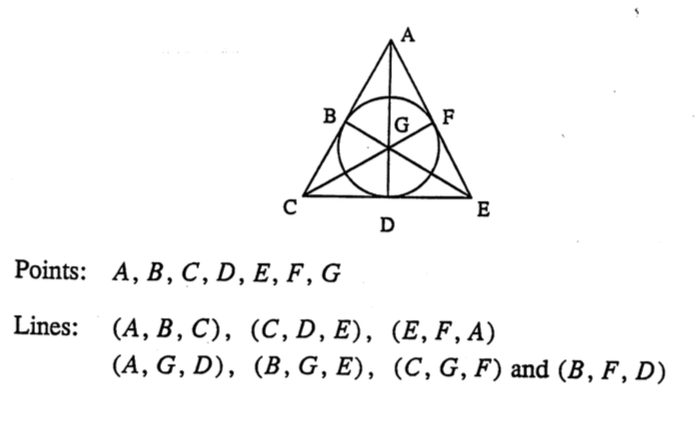
\includegraphics[scale=0.3]{Fano.png}
\caption{Fano Geometry}
\end{figure}
\end{frame}



\begin{frame}{LU decomposition}
A 2009 undergraduate thesis by A Patil studies LU decomposition. He compares 3 cases:
\begin{itemize}
\item Full mesh network with 144 nodes
\item $\mathbb{P}_4(2)$ with 155 nodes with two data layouts
\end{itemize}

Conclusions are that $PG$ computations are not much slower than full mesh and utilize resources much better.  Much more work needs to be done in studies like this.

\end{frame}


\section{Network Topology \& Implementation}

\begin{frame}{Network Topology}

\begin{itemize}
\item The full network defined by incidence of memory modules $M\in\Omeage_m$ in processors $P\in\Omega_p$ has beautiful properties: e.g. for $d==2,4$ any two processors are separated by at most 2,4 hops.
\item If only perfect patterns are used for communication and a switch can be programmed to set up the required connections then only one connection per memory module is needed and a congestion free network with uniform latency arises.
\end{itemize}

\end{frame}

\begin{frame}{Quantum Electron Tunneling Networks}
\begin{figure}
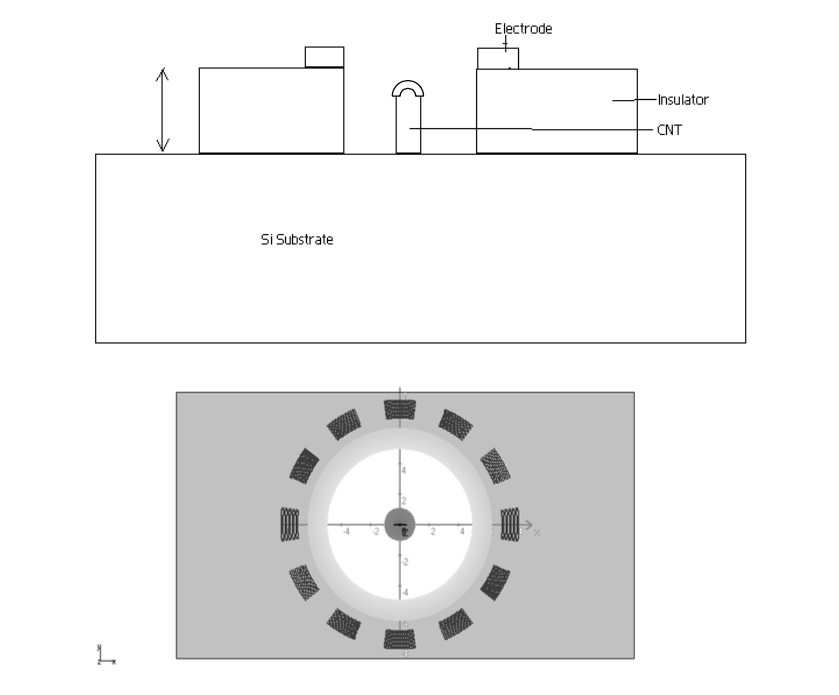
\includegraphics[scale=0.2]{nanocb-nic.png}
\caption{Carbon Nano Tube Network Emittor}
\end{figure}
\end{frame}

\begin{frame}{Perfect Pattern and Tunneling Networks}
\begin{figure}
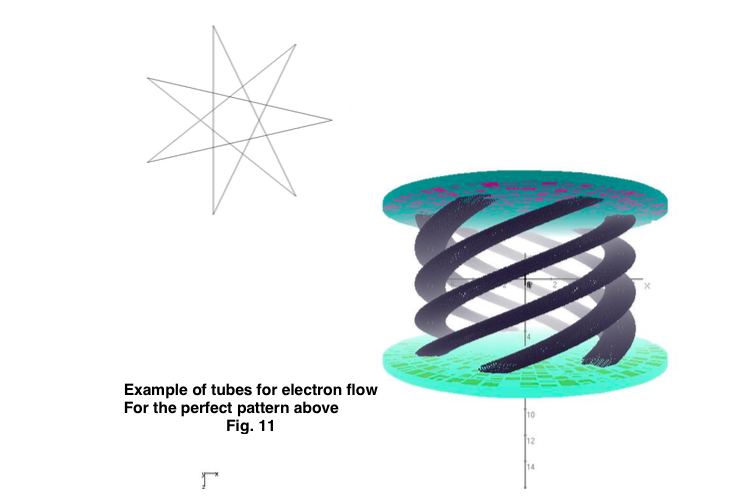
\includegraphics[scale=0.41]{cylinder-pattern.png}
\caption{EM field changing routing}
\end{figure}
\end{frame}

\begin{frame}{Projective Difference Networks}




\end{frame}



\section{Commercial Turbulence}

\begin{frame}{Who is Narendra Karmarkar}
\begin{itemize}
\item Invented a famous new linear programming algorithm in 80's
\item Then published ~5 papers 1989-1994 about a new parallel architecture
\item In 2005 TATA founded CRL in Pune to commercialize the architecture
\item A year later, Karmarkar had left, CRL looked only at it a little
\item Karmarkar is now an independent consultant in India
\item Since 2009 I have been interested in this. 
\end{itemize}
\end{frame}

\begin{frame}{A mathematical approach to developing parallel algorithms}
\begin{block}{
Global parallel instructions and sequences of such instructions}
\begin{itemize}
\item Derived from mathematical symmetries of the problem and architecture
\item Limited concurrency
\item Good load balancing
\item No contention for network and memory 
\item A method ("compiler") to apply this
\end{itemize}
\end{block}
\end{frame}

\begin{frame}{Application}

\begin{block}{Promise of the software methodology}
\begin{itemize}
\item Applied to a very limited set of problems - promising
\item The symmetry group is the crux, not specific hardware
\item The optimizations connect data-centric and instruction-centric approach
\end{itemize}
\end{block}
\begin{block}{Hardware}
\begin{itemize}
\item Older ideas from the 1990's
\item Radically new ideas involving nano-technology
\item Can be explored on lots of hardware (e.g. SMP, SOC, Cluster)
\end{itemize}
\end{block}
\end{frame}

\begin{frame}{The scientific state of the concepts}

\begin{block}{Key ideas seem sound}
\begin{itemize}
\item Mathematics for construction of parallel programs
\item The network topology
\item A few important examples
\item Various extensions seem sound (e.g. re-compute vs memory tradeoff)
\end{itemize}
\end{block}
\end{frame}

\begin{frame}{However ...}
\begin{block}{Details are lacking}
\begin{itemize}
\item The compiler is under-specified but has potential
\item Even the simplest examples are not reproducible due to lack of source
\item Missing complexity computations and benchmarking
\item Realistic performance cost functions likely to be very hardware sensitive
\item It's pretty important to test for wider applicability
\begin{enumerate}
\item Ambitious ones: e.g. produce parallel Prolog programs
\item Modest ones: programs with different data access patterns
\end{enumerate}
\end{itemize}
\end{block}
\end{frame}

\begin{frame}{What has been done commercially}
\begin{itemize}
\item We don't know everything - secrets abound
\item CRL had a concrete idea how to exploit the network topology
\item Possibly others have tried to look at this
\item It's probably not ready for industry but a very promising research project
\end{itemize}
\end{frame}



\section{The compiler}
\begin{frame}{A few notes about the compiler}
\begin{itemize}
\item A paper from 1990 outlines how to create a compiler
\item The compiler uses the data layout as input
\item Then proceeds in a relatively straightforward fashion to derive perfect parallel access patterns from the program's data flow graph
\item Possibly a better compiler design would compute the optimal data layout
\end{itemize}
\end{frame}

\section{A nano-vacuum electronics network}

\begin{frame}{Application - Hardware}
\begin{itemize}
\item
In the older papers (~1990) Karmarkar described pretty complete hardware architecture.  May be good, probably not economical.
\item
In 2008 he published ideas using nano-vacuum electronics to package the architecture in a radically different manner.
\item
Think of a cylinder with 1000's of cores on the surface and a quantum electron tunneling network connecting them.
\item
Key property of the network is extremely high bandwidth, latency governed by speed of light and electronics. Reactivity of emittor ~ Femto seconds
\end{itemize}
\end{frame}




\section{Conclusions}
\begin{frame}{Conclusions}
\begin{itemize}
\item Possibly this is very novel (even though it's 25 years old!)
\item A very unusual combination of mathematics, physics and parallel programming
\item There is plenty of opportunity to explore this
\item I plan to publish a small program to remove initial hurdles, e.g. a software simulator for PG machines that is somewhat programmable
\item Nobody knows what the conclusions will really be.
\item Up to now I think all ideas come from Narendra Karmarkar and his collaborators
\end{itemize}
\end{frame}


\begin{frame}
  \frametitle{Thank you!}
\end{frame}
\end{document}
